\documentclass[1p]{elsarticle_modified}
%\bibliographystyle{elsarticle-num}

%\usepackage[colorlinks]{hyperref}
%\usepackage{abbrmath_seonhwa} %\Abb, \Ascr, \Acal ,\Abf, \Afrak
\usepackage{amsfonts}
\usepackage{amssymb}
\usepackage{amsmath}
\usepackage{amsthm}
\usepackage{scalefnt}
\usepackage{amsbsy}
\usepackage{kotex}
\usepackage{caption}
\usepackage{subfig}
\usepackage{color}
\usepackage{graphicx}
\usepackage{xcolor} %% white, black, red, green, blue, cyan, magenta, yellow
\usepackage{float}
\usepackage{setspace}
\usepackage{hyperref}

\usepackage{tikz}
\usetikzlibrary{arrows}

\usepackage{multirow}
\usepackage{array} % fixed length table
\usepackage{hhline}

%%%%%%%%%%%%%%%%%%%%%
\makeatletter
\renewcommand*\env@matrix[1][\arraystretch]{%
	\edef\arraystretch{#1}%
	\hskip -\arraycolsep
	\let\@ifnextchar\new@ifnextchar
	\array{*\c@MaxMatrixCols c}}
\makeatother %https://tex.stackexchange.com/questions/14071/how-can-i-increase-the-line-spacing-in-a-matrix
%%%%%%%%%%%%%%%

\usepackage[normalem]{ulem}

\newcommand{\msout}[1]{\ifmmode\text{\sout{\ensuremath{#1}}}\else\sout{#1}\fi}
%SOURCE: \msout is \stkout macro in https://tex.stackexchange.com/questions/20609/strikeout-in-math-mode

\newcommand{\cancel}[1]{
	\ifmmode
	{\color{red}\msout{#1}}
	\else
	{\color{red}\sout{#1}}
	\fi
}

\newcommand{\add}[1]{
	{\color{blue}\uwave{#1}}
}

\newcommand{\replace}[2]{
	\ifmmode
	{\color{red}\msout{#1}}{\color{blue}\uwave{#2}}
	\else
	{\color{red}\sout{#1}}{\color{blue}\uwave{#2}}
	\fi
}

\newcommand{\Sol}{\mathcal{S}} %segment
\newcommand{\D}{D} %diagram
\newcommand{\A}{\mathcal{A}} %arc


%%%%%%%%%%%%%%%%%%%%%%%%%%%%%5 test

\def\sl{\operatorname{\textup{SL}}(2,\Cbb)}
\def\psl{\operatorname{\textup{PSL}}(2,\Cbb)}
\def\quan{\mkern 1mu \triangleright \mkern 1mu}

\theoremstyle{definition}
\newtheorem{thm}{Theorem}[section]
\newtheorem{prop}[thm]{Proposition}
\newtheorem{lem}[thm]{Lemma}
\newtheorem{ques}[thm]{Question}
\newtheorem{cor}[thm]{Corollary}
\newtheorem{defn}[thm]{Definition}
\newtheorem{exam}[thm]{Example}
\newtheorem{rmk}[thm]{Remark}
\newtheorem{alg}[thm]{Algorithm}

\newcommand{\I}{\sqrt{-1}}
\begin{document}

%\begin{frontmatter}
%
%\title{Boundary parabolic representations of knots up to 8 crossings}
%
%%% Group authors per affiliation:
%\author{Yunhi Cho} 
%\address{Department of Mathematics, University of Seoul, Seoul, Korea}
%\ead{yhcho@uos.ac.kr}
%
%
%\author{Seonhwa Kim} %\fnref{s_kim}}
%\address{Center for Geometry and Physics, Institute for Basic Science, Pohang, 37673, Korea}
%\ead{ryeona17@ibs.re.kr}
%
%\author{Hyuk Kim}
%\address{Department of Mathematical Sciences, Seoul National University, Seoul 08826, Korea}
%\ead{hyukkim@snu.ac.kr}
%
%\author{Seokbeom Yoon}
%\address{Department of Mathematical Sciences, Seoul National University, Seoul, 08826,  Korea}
%\ead{sbyoon15@snu.ac.kr}
%
%\begin{abstract}
%We find all boundary parabolic representation of knots up to 8 crossings.
%
%\end{abstract}
%\begin{keyword}
%    \MSC[2010] 57M25 
%\end{keyword}
%
%\end{frontmatter}

%\linenumbers
%\tableofcontents
%
\newcommand\colored[1]{\textcolor{white}{\rule[-0.35ex]{0.8em}{1.4ex}}\kern-0.8em\color{red} #1}%
%\newcommand\colored[1]{\textcolor{white}{ #1}\kern-2.17ex	\textcolor{white}{ #1}\kern-1.81ex	\textcolor{white}{ #1}\kern-2.15ex\color{red}#1	}

{\Large $\underline{12n_{0298}~(K12n_{0298})}$}

\setlength{\tabcolsep}{10pt}
\renewcommand{\arraystretch}{1.6}
\vspace{1cm}\begin{tabular}{m{100pt}>{\centering\arraybackslash}m{274pt}}
\multirow{5}{120pt}{
	\centering
	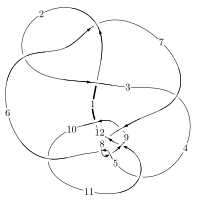
\includegraphics[width=112pt]{../../../GIT/diagram.site/Diagrams/png/2387_12n_0298.png}\\
\ \ \ A knot diagram\footnotemark}&
\allowdisplaybreaks
\textbf{Linearized knot diagam} \\
\cline{2-2}
 &
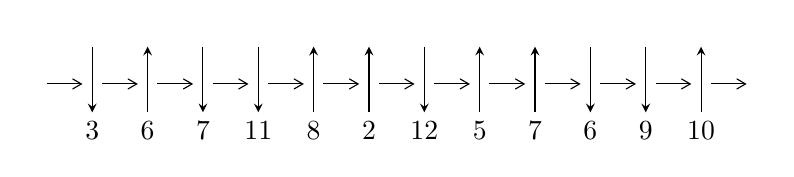
\begin{tikzpicture}[x=20pt, y=17pt]
	% nodes
	\node (C0) at (0, 0) {};
	\node (C1) at (1, 0) {};
	\node (C1U) at (1, +1) {};
	\node (C1D) at (1, -1) {3};

	\node (C2) at (2, 0) {};
	\node (C2U) at (2, +1) {};
	\node (C2D) at (2, -1) {6};

	\node (C3) at (3, 0) {};
	\node (C3U) at (3, +1) {};
	\node (C3D) at (3, -1) {7};

	\node (C4) at (4, 0) {};
	\node (C4U) at (4, +1) {};
	\node (C4D) at (4, -1) {11};

	\node (C5) at (5, 0) {};
	\node (C5U) at (5, +1) {};
	\node (C5D) at (5, -1) {8};

	\node (C6) at (6, 0) {};
	\node (C6U) at (6, +1) {};
	\node (C6D) at (6, -1) {2};

	\node (C7) at (7, 0) {};
	\node (C7U) at (7, +1) {};
	\node (C7D) at (7, -1) {12};

	\node (C8) at (8, 0) {};
	\node (C8U) at (8, +1) {};
	\node (C8D) at (8, -1) {5};

	\node (C9) at (9, 0) {};
	\node (C9U) at (9, +1) {};
	\node (C9D) at (9, -1) {7};

	\node (C10) at (10, 0) {};
	\node (C10U) at (10, +1) {};
	\node (C10D) at (10, -1) {6};

	\node (C11) at (11, 0) {};
	\node (C11U) at (11, +1) {};
	\node (C11D) at (11, -1) {9};

	\node (C12) at (12, 0) {};
	\node (C12U) at (12, +1) {};
	\node (C12D) at (12, -1) {10};
	\node (C13) at (13, 0) {};

	% arrows
	\draw[->,>={angle 60}]
	(C0) edge (C1) (C1) edge (C2) (C2) edge (C3) (C3) edge (C4) (C4) edge (C5) (C5) edge (C6) (C6) edge (C7) (C7) edge (C8) (C8) edge (C9) (C9) edge (C10) (C10) edge (C11) (C11) edge (C12) (C12) edge (C13) ;	\draw[->,>=stealth]
	(C1U) edge (C1D) (C2D) edge (C2U) (C3U) edge (C3D) (C4U) edge (C4D) (C5D) edge (C5U) (C6D) edge (C6U) (C7U) edge (C7D) (C8D) edge (C8U) (C9D) edge (C9U) (C10U) edge (C10D) (C11U) edge (C11D) (C12D) edge (C12U) ;
	\end{tikzpicture} \\
\hhline{~~} \\& 
\textbf{Solving Sequence} \\ \cline{2-2} 
 &
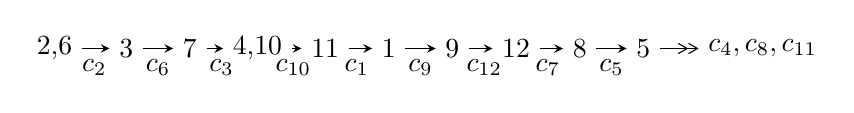
\begin{tikzpicture}[x=23pt, y=7pt]
	% node
	\node (A0) at (-1/8, 0) {2,6};
	\node (A1) at (1, 0) {3};
	\node (A2) at (2, 0) {7};
	\node (A3) at (49/16, 0) {4,10};
	\node (A4) at (33/8, 0) {11};
	\node (A5) at (41/8, 0) {1};
	\node (A6) at (49/8, 0) {9};
	\node (A7) at (57/8, 0) {12};
	\node (A8) at (65/8, 0) {8};
	\node (A9) at (73/8, 0) {5};
	\node (C1) at (1/2, -1) {$c_{2}$};
	\node (C2) at (3/2, -1) {$c_{6}$};
	\node (C3) at (5/2, -1) {$c_{3}$};
	\node (C4) at (29/8, -1) {$c_{10}$};
	\node (C5) at (37/8, -1) {$c_{1}$};
	\node (C6) at (45/8, -1) {$c_{9}$};
	\node (C7) at (53/8, -1) {$c_{12}$};
	\node (C8) at (61/8, -1) {$c_{7}$};
	\node (C9) at (69/8, -1) {$c_{5}$};
	\node (A10) at (11, 0) {$c_{4},c_{8},c_{11}$};

	% edge
	\draw[->,>=stealth]	
	(A0) edge (A1) (A1) edge (A2) (A2) edge (A3) (A3) edge (A4) (A4) edge (A5) (A5) edge (A6) (A6) edge (A7) (A7) edge (A8) (A8) edge (A9) ;
	\draw[->>,>={angle 60}]	
	(A9) edge (A10);
\end{tikzpicture} \\ 

\end{tabular} \\

\footnotetext{
The image of knot diagram is generated by the software ``\textbf{Draw programme}" developed by Andrew Bartholomew(\url{http://www.layer8.co.uk/maths/draw/index.htm\#Running-draw}), where we modified some parts for our purpose(\url{https://github.com/CATsTAILs/LinksPainter}).
}\phantom \\ \newline 
\centering \textbf{Ideals for irreducible components\footnotemark of $X_{\text{par}}$} 
 
\begin{align*}
I^u_{1}&=\langle 
1.39637\times10^{86} u^{63}+5.43528\times10^{86} u^{62}+\cdots+2.96182\times10^{85} b-1.86518\times10^{86},\\
\phantom{I^u_{1}}&\phantom{= \langle  }-2.24145\times10^{86} u^{63}-9.03174\times10^{86} u^{62}+\cdots+2.96182\times10^{85} a-2.29298\times10^{85},\;u^{64}+4 u^{63}+\cdots-4 u+1\rangle \\
I^u_{2}&=\langle 
2 u^{19}+7 u^{17}+\cdots+b-4 u,\;-2 u^{19}+u^{18}+\cdots+a-1,\;u^{20}- u^{19}+\cdots-2 u+1\rangle \\
\\
\end{align*}
\raggedright * 2 irreducible components of $\dim_{\mathbb{C}}=0$, with total 84 representations.\\
\footnotetext{All coefficients of polynomials are rational numbers. But the coefficients are sometimes approximated in decimal forms when there is not enough margin.}
\newpage
\renewcommand{\arraystretch}{1}
\centering \section*{I. $I^u_{1}= \langle 1.40\times10^{86} u^{63}+5.44\times10^{86} u^{62}+\cdots+2.96\times10^{85} b-1.87\times10^{86},\;-2.24\times10^{86} u^{63}-9.03\times10^{86} u^{62}+\cdots+2.96\times10^{85} a-2.29\times10^{85},\;u^{64}+4 u^{63}+\cdots-4 u+1 \rangle$}
\flushleft \textbf{(i) Arc colorings}\\
\begin{tabular}{m{7pt} m{180pt} m{7pt} m{180pt} }
\flushright $a_{2}=$&$\begin{pmatrix}1\\0\end{pmatrix}$ \\
\flushright $a_{6}=$&$\begin{pmatrix}0\\u\end{pmatrix}$ \\
\flushright $a_{3}=$&$\begin{pmatrix}1\\- u^2\end{pmatrix}$ \\
\flushright $a_{7}=$&$\begin{pmatrix}u\\u\end{pmatrix}$ \\
\flushright $a_{4}=$&$\begin{pmatrix}u^4+u^2+1\\u^4\end{pmatrix}$ \\
\flushright $a_{10}=$&$\begin{pmatrix}7.56782 u^{63}+30.4939 u^{62}+\cdots+24.0222 u+0.774178\\-4.71457 u^{63}-18.3512 u^{62}+\cdots-27.2378 u+6.29741\end{pmatrix}$ \\
\flushright $a_{11}=$&$\begin{pmatrix}7.56782 u^{63}+30.4939 u^{62}+\cdots+24.0222 u+0.774178\\-6.38660 u^{63}-24.4128 u^{62}+\cdots-33.9152 u+6.07481\end{pmatrix}$ \\
\flushright $a_{1}=$&$\begin{pmatrix}u^2+1\\- u^4\end{pmatrix}$ \\
\flushright $a_{9}=$&$\begin{pmatrix}3.86933 u^{63}+16.0937 u^{62}+\cdots+10.6018 u+1.05869\\-8.41306 u^{63}-32.7513 u^{62}+\cdots-40.6582 u+6.58192\end{pmatrix}$ \\
\flushright $a_{12}=$&$\begin{pmatrix}6.42367 u^{63}+32.1547 u^{62}+\cdots-45.0142 u+17.0072\\3.79100 u^{63}+16.1352 u^{62}+\cdots+0.840596 u+4.38519\end{pmatrix}$ \\
\flushright $a_{8}=$&$\begin{pmatrix}0.562618 u^{63}+2.63121 u^{62}+\cdots-36.1172 u+8.44512\\4.32626 u^{63}+17.5719 u^{62}+\cdots+18.4608 u-1.19617\end{pmatrix}$ \\
\flushright $a_{5}=$&$\begin{pmatrix}5.84919 u^{63}+21.5137 u^{62}+\cdots+53.4241 u-7.65911\\1.92460 u^{63}+7.73661 u^{62}+\cdots+10.1183 u-1.34592\end{pmatrix}$\\&\end{tabular}
\flushleft \textbf{(ii) Obstruction class $= -1$}\\~\\
\flushleft \textbf{(iii) Cusp Shapes $= 30.7036 u^{63}+141.686 u^{62}+\cdots-73.0395 u+38.2307$}\\~\\
\newpage\renewcommand{\arraystretch}{1}
\flushleft \textbf{(iv) u-Polynomials at the component}\newline \\
\begin{tabular}{m{50pt}|m{274pt}}
Crossings & \hspace{64pt}u-Polynomials at each crossing \\
\hline $$\begin{aligned}c_{1}\end{aligned}$$&$\begin{aligned}
&u^{64}+14 u^{63}+\cdots+30 u+1
\end{aligned}$\\
\hline $$\begin{aligned}c_{2},c_{6}\end{aligned}$$&$\begin{aligned}
&u^{64}-4 u^{63}+\cdots+4 u+1
\end{aligned}$\\
\hline $$\begin{aligned}c_{3}\end{aligned}$$&$\begin{aligned}
&u^{64}+4 u^{63}+\cdots-4232566 u+8381893
\end{aligned}$\\
\hline $$\begin{aligned}c_{4}\end{aligned}$$&$\begin{aligned}
&u^{64}+3 u^{63}+\cdots-317686 u+108431
\end{aligned}$\\
\hline $$\begin{aligned}c_{5},c_{8}\end{aligned}$$&$\begin{aligned}
&u^{64}+u^{63}+\cdots+8 u^2+1
\end{aligned}$\\
\hline $$\begin{aligned}c_{7}\end{aligned}$$&$\begin{aligned}
&u^{64}+3 u^{63}+\cdots-14 u+1
\end{aligned}$\\
\hline $$\begin{aligned}c_{9}\end{aligned}$$&$\begin{aligned}
&u^{64}+15 u^{63}+\cdots+1193304 u+134569
\end{aligned}$\\
\hline $$\begin{aligned}c_{10}\end{aligned}$$&$\begin{aligned}
&u^{64}+2 u^{63}+\cdots-28804 u+319
\end{aligned}$\\
\hline $$\begin{aligned}c_{11}\end{aligned}$$&$\begin{aligned}
&u^{64}-13 u^{63}+\cdots-516 u+31
\end{aligned}$\\
\hline $$\begin{aligned}c_{12}\end{aligned}$$&$\begin{aligned}
&u^{64}-11 u^{63}+\cdots+4233776 u+540971
\end{aligned}$\\
\hline
\end{tabular}\\~\\
\newpage\renewcommand{\arraystretch}{1}
\flushleft \textbf{(v) Riley Polynomials at the component}\newline \\
\begin{tabular}{m{50pt}|m{274pt}}
Crossings & \hspace{64pt}Riley Polynomials at each crossing \\
\hline $$\begin{aligned}c_{1}\end{aligned}$$&$\begin{aligned}
&y^{64}+82 y^{63}+\cdots+154 y+1
\end{aligned}$\\
\hline $$\begin{aligned}c_{2},c_{6}\end{aligned}$$&$\begin{aligned}
&y^{64}+14 y^{63}+\cdots+30 y+1
\end{aligned}$\\
\hline $$\begin{aligned}c_{3}\end{aligned}$$&$\begin{aligned}
&y^{64}+162 y^{63}+\cdots+4185418110089892 y+70256130263449
\end{aligned}$\\
\hline $$\begin{aligned}c_{4}\end{aligned}$$&$\begin{aligned}
&y^{64}+29 y^{63}+\cdots+248335976782 y+11757281761
\end{aligned}$\\
\hline $$\begin{aligned}c_{5},c_{8}\end{aligned}$$&$\begin{aligned}
&y^{64}+43 y^{63}+\cdots+16 y+1
\end{aligned}$\\
\hline $$\begin{aligned}c_{7}\end{aligned}$$&$\begin{aligned}
&y^{64}+5 y^{63}+\cdots-30 y+1
\end{aligned}$\\
\hline $$\begin{aligned}c_{9}\end{aligned}$$&$\begin{aligned}
&y^{64}-59 y^{63}+\cdots-87140422306 y+18108815761
\end{aligned}$\\
\hline $$\begin{aligned}c_{10}\end{aligned}$$&$\begin{aligned}
&y^{64}+100 y^{63}+\cdots-262631966 y+101761
\end{aligned}$\\
\hline $$\begin{aligned}c_{11}\end{aligned}$$&$\begin{aligned}
&y^{64}+y^{63}+\cdots+5676 y+961
\end{aligned}$\\
\hline $$\begin{aligned}c_{12}\end{aligned}$$&$\begin{aligned}
&y^{64}-91 y^{63}+\cdots-7005093425444 y+292649622841
\end{aligned}$\\
\hline
\end{tabular}\\~\\
\newpage\flushleft \textbf{(vi) Complex Volumes and Cusp Shapes}
$$\begin{array}{c|c|c}  
\text{Solutions to }I^u_{1}& \I (\text{vol} + \sqrt{-1}CS) & \text{Cusp shape}\\
 \hline 
\begin{aligned}
u &= \phantom{-}0.939075 + 0.271602 I \\
a &= \phantom{-}0.482093 - 0.464401 I \\
b &= -0.755445 - 0.284336 I\end{aligned}
 & -0.44441 - 3.98622 I & \phantom{-0.000000 } 0 \\ \hline\begin{aligned}
u &= \phantom{-}0.939075 - 0.271602 I \\
a &= \phantom{-}0.482093 + 0.464401 I \\
b &= -0.755445 + 0.284336 I\end{aligned}
 & -0.44441 + 3.98622 I & \phantom{-0.000000 } 0 \\ \hline\begin{aligned}
u &= -0.722916 + 0.601079 I \\
a &= \phantom{-}0.123478 - 0.330623 I \\
b &= \phantom{-}1.32766 - 0.80295 I\end{aligned}
 & -1.03187 - 6.00979 I & \phantom{-0.000000 -}0. + 8.60089 I \\ \hline\begin{aligned}
u &= -0.722916 - 0.601079 I \\
a &= \phantom{-}0.123478 + 0.330623 I \\
b &= \phantom{-}1.32766 + 0.80295 I\end{aligned}
 & -1.03187 + 6.00979 I & \phantom{-0.000000 } 0. - 8.60089 I \\ \hline\begin{aligned}
u &= -0.432677 + 0.976451 I \\
a &= \phantom{-}0.843388 - 0.347446 I \\
b &= \phantom{-}0.197103 + 0.398413 I\end{aligned}
 & -2.46162 + 1.46729 I & \phantom{-0.000000 } 0 \\ \hline\begin{aligned}
u &= -0.432677 - 0.976451 I \\
a &= \phantom{-}0.843388 + 0.347446 I \\
b &= \phantom{-}0.197103 - 0.398413 I\end{aligned}
 & -2.46162 - 1.46729 I & \phantom{-0.000000 } 0 \\ \hline\begin{aligned}
u &= \phantom{-}0.194061 + 1.056770 I \\
a &= \phantom{-}0.586720 + 0.232918 I \\
b &= \phantom{-}0.052356 - 0.350919 I\end{aligned}
 & -1.71226 + 0.14587 I & \phantom{-0.000000 } 0 \\ \hline\begin{aligned}
u &= \phantom{-}0.194061 - 1.056770 I \\
a &= \phantom{-}0.586720 - 0.232918 I \\
b &= \phantom{-}0.052356 + 0.350919 I\end{aligned}
 & -1.71226 - 0.14587 I & \phantom{-0.000000 } 0 \\ \hline\begin{aligned}
u &= -0.475448 + 0.789845 I \\
a &= \phantom{-}0.290628 - 0.808412 I \\
b &= \phantom{-}0.868055 - 0.780912 I\end{aligned}
 & \phantom{-}0.01302 - 1.90453 I & \phantom{-0.000000 -}0. + 2.57583 I \\ \hline\begin{aligned}
u &= -0.475448 - 0.789845 I \\
a &= \phantom{-}0.290628 + 0.808412 I \\
b &= \phantom{-}0.868055 + 0.780912 I\end{aligned}
 & \phantom{-}0.01302 + 1.90453 I & \phantom{-0.000000 } 0. - 2.57583 I\\
 \hline 
 \end{array}$$\newpage$$\begin{array}{c|c|c}  
\text{Solutions to }I^u_{1}& \I (\text{vol} + \sqrt{-1}CS) & \text{Cusp shape}\\
 \hline 
\begin{aligned}
u &= -0.791240 + 0.428776 I \\
a &= \phantom{-}0.912391 + 1.040550 I \\
b &= -0.676221 + 0.565206 I\end{aligned}
 & \phantom{-}2.49559 - 1.05555 I & \phantom{-}7.00649 + 1.32061 I \\ \hline\begin{aligned}
u &= -0.791240 - 0.428776 I \\
a &= \phantom{-}0.912391 - 1.040550 I \\
b &= -0.676221 - 0.565206 I\end{aligned}
 & \phantom{-}2.49559 + 1.05555 I & \phantom{-}7.00649 - 1.32061 I \\ \hline\begin{aligned}
u &= \phantom{-}0.400359 + 0.788642 I \\
a &= -0.069876 + 1.329720 I \\
b &= \phantom{-}1.035650 + 0.916049 I\end{aligned}
 & -0.52477 + 4.45766 I & -3.10979 - 9.91982 I \\ \hline\begin{aligned}
u &= \phantom{-}0.400359 - 0.788642 I \\
a &= -0.069876 - 1.329720 I \\
b &= \phantom{-}1.035650 - 0.916049 I\end{aligned}
 & -0.52477 - 4.45766 I & -3.10979 + 9.91982 I \\ \hline\begin{aligned}
u &= \phantom{-}0.299647 + 0.825342 I \\
a &= -0.912074 + 0.700445 I \\
b &= -1.95342 + 1.10428 I\end{aligned}
 & -3.49922 - 2.68192 I & -5.19582 + 0.87569 I \\ \hline\begin{aligned}
u &= \phantom{-}0.299647 - 0.825342 I \\
a &= -0.912074 - 0.700445 I \\
b &= -1.95342 - 1.10428 I\end{aligned}
 & -3.49922 + 2.68192 I & -5.19582 - 0.87569 I \\ \hline\begin{aligned}
u &= \phantom{-}0.589193 + 0.551154 I \\
a &= \phantom{-}0.85587 - 2.43022 I \\
b &= -0.536571 - 0.801267 I\end{aligned}
 & -2.27399 + 6.14015 I & \phantom{-}2.22329 - 10.33949 I \\ \hline\begin{aligned}
u &= \phantom{-}0.589193 - 0.551154 I \\
a &= \phantom{-}0.85587 + 2.43022 I \\
b &= -0.536571 + 0.801267 I\end{aligned}
 & -2.27399 - 6.14015 I & \phantom{-}2.22329 + 10.33949 I \\ \hline\begin{aligned}
u &= \phantom{-}0.274975 + 1.168590 I \\
a &= -0.0110651 + 0.0113996 I \\
b &= -0.306856 + 0.642395 I\end{aligned}
 & -5.23856 - 0.57022 I & \phantom{-0.000000 } 0 \\ \hline\begin{aligned}
u &= \phantom{-}0.274975 - 1.168590 I \\
a &= -0.0110651 - 0.0113996 I \\
b &= -0.306856 - 0.642395 I\end{aligned}
 & -5.23856 + 0.57022 I & \phantom{-0.000000 } 0\\
 \hline 
 \end{array}$$\newpage$$\begin{array}{c|c|c}  
\text{Solutions to }I^u_{1}& \I (\text{vol} + \sqrt{-1}CS) & \text{Cusp shape}\\
 \hline 
\begin{aligned}
u &= -0.457124 + 1.152150 I \\
a &= -0.645292 - 0.183503 I \\
b &= -1.24538 - 1.10620 I\end{aligned}
 & -0.02531 - 3.74403 I & \phantom{-0.000000 } 0 \\ \hline\begin{aligned}
u &= -0.457124 - 1.152150 I \\
a &= -0.645292 + 0.183503 I \\
b &= -1.24538 + 1.10620 I\end{aligned}
 & -0.02531 + 3.74403 I & \phantom{-0.000000 } 0 \\ \hline\begin{aligned}
u &= -0.879640 + 0.881204 I \\
a &= -0.79455 + 1.61194 I \\
b &= -1.45624 + 0.94426 I\end{aligned}
 & \phantom{-}6.66965 - 5.86737 I & \phantom{-0.000000 } 0 \\ \hline\begin{aligned}
u &= -0.879640 - 0.881204 I \\
a &= -0.79455 - 1.61194 I \\
b &= -1.45624 - 0.94426 I\end{aligned}
 & \phantom{-}6.66965 + 5.86737 I & \phantom{-0.000000 } 0 \\ \hline\begin{aligned}
u &= -0.838867 + 0.958647 I \\
a &= -1.35935 + 0.86354 I \\
b &= -1.99957 + 0.33680 I\end{aligned}
 & \phantom{-}6.41424 - 0.52117 I & \phantom{-0.000000 } 0 \\ \hline\begin{aligned}
u &= -0.838867 - 0.958647 I \\
a &= -1.35935 - 0.86354 I \\
b &= -1.99957 - 0.33680 I\end{aligned}
 & \phantom{-}6.41424 + 0.52117 I & \phantom{-0.000000 } 0 \\ \hline\begin{aligned}
u &= \phantom{-}0.897037 + 0.932073 I \\
a &= -1.13339 - 1.29721 I \\
b &= -1.76535 - 0.72437 I\end{aligned}
 & \phantom{-}8.51868 + 3.30961 I & \phantom{-0.000000 } 0 \\ \hline\begin{aligned}
u &= \phantom{-}0.897037 - 0.932073 I \\
a &= -1.13339 + 1.29721 I \\
b &= -1.76535 + 0.72437 I\end{aligned}
 & \phantom{-}8.51868 - 3.30961 I & \phantom{-0.000000 } 0 \\ \hline\begin{aligned}
u &= \phantom{-}0.530563 + 0.465648 I \\
a &= -0.472852 + 0.171059 I \\
b &= \phantom{-}1.121760 + 0.641421 I\end{aligned}
 & \phantom{-}0.55435 + 2.88435 I & \phantom{-}4.59418 - 0.12217 I \\ \hline\begin{aligned}
u &= \phantom{-}0.530563 - 0.465648 I \\
a &= -0.472852 - 0.171059 I \\
b &= \phantom{-}1.121760 - 0.641421 I\end{aligned}
 & \phantom{-}0.55435 - 2.88435 I & \phantom{-}4.59418 + 0.12217 I\\
 \hline 
 \end{array}$$\newpage$$\begin{array}{c|c|c}  
\text{Solutions to }I^u_{1}& \I (\text{vol} + \sqrt{-1}CS) & \text{Cusp shape}\\
 \hline 
\begin{aligned}
u &= -0.385835 + 0.588474 I \\
a &= \phantom{-}0.836666 - 0.736399 I \\
b &= \phantom{-}0.811989 - 0.180829 I\end{aligned}
 & \phantom{-}0.38260 - 1.61712 I & \phantom{-}2.69865 + 4.73413 I \\ \hline\begin{aligned}
u &= -0.385835 - 0.588474 I \\
a &= \phantom{-}0.836666 + 0.736399 I \\
b &= \phantom{-}0.811989 + 0.180829 I\end{aligned}
 & \phantom{-}0.38260 + 1.61712 I & \phantom{-}2.69865 - 4.73413 I \\ \hline\begin{aligned}
u &= -1.026810 + 0.827404 I \\
a &= -0.507979 + 1.128420 I \\
b &= -1.29031 + 0.58664 I\end{aligned}
 & \phantom{-}7.40053 - 0.12600 I & \phantom{-0.000000 } 0 \\ \hline\begin{aligned}
u &= -1.026810 - 0.827404 I \\
a &= -0.507979 - 1.128420 I \\
b &= -1.29031 - 0.58664 I\end{aligned}
 & \phantom{-}7.40053 + 0.12600 I & \phantom{-0.000000 } 0 \\ \hline\begin{aligned}
u &= \phantom{-}0.488940 + 1.231620 I \\
a &= -0.531491 - 0.111009 I \\
b &= -1.041740 + 0.612916 I\end{aligned}
 & -3.67677 + 9.30666 I & \phantom{-0.000000 } 0 \\ \hline\begin{aligned}
u &= \phantom{-}0.488940 - 1.231620 I \\
a &= -0.531491 + 0.111009 I \\
b &= -1.041740 - 0.612916 I\end{aligned}
 & -3.67677 - 9.30666 I & \phantom{-0.000000 } 0 \\ \hline\begin{aligned}
u &= -0.063841 + 0.650559 I \\
a &= \phantom{-}0.415319 - 0.941017 I \\
b &= -0.556116 - 1.216000 I\end{aligned}
 & -1.14528 - 1.52727 I & -4.52889 + 4.44249 I \\ \hline\begin{aligned}
u &= -0.063841 - 0.650559 I \\
a &= \phantom{-}0.415319 + 0.941017 I \\
b &= -0.556116 + 1.216000 I\end{aligned}
 & -1.14528 + 1.52727 I & -4.52889 - 4.44249 I \\ \hline\begin{aligned}
u &= -1.037000 + 0.860981 I \\
a &= \phantom{-}1.10948 - 1.12589 I \\
b &= \phantom{-}1.60768 + 0.28265 I\end{aligned}
 & \phantom{-}7.61657 + 8.96188 I & \phantom{-0.000000 } 0 \\ \hline\begin{aligned}
u &= -1.037000 - 0.860981 I \\
a &= \phantom{-}1.10948 + 1.12589 I \\
b &= \phantom{-}1.60768 - 0.28265 I\end{aligned}
 & \phantom{-}7.61657 - 8.96188 I & \phantom{-0.000000 } 0\\
 \hline 
 \end{array}$$\newpage$$\begin{array}{c|c|c}  
\text{Solutions to }I^u_{1}& \I (\text{vol} + \sqrt{-1}CS) & \text{Cusp shape}\\
 \hline 
\begin{aligned}
u &= \phantom{-}1.026730 + 0.876368 I \\
a &= \phantom{-}1.16571 + 1.14718 I \\
b &= \phantom{-}1.66461 - 0.43980 I\end{aligned}
 & \phantom{-}11.07350 - 2.80334 I & \phantom{-0.000000 } 0 \\ \hline\begin{aligned}
u &= \phantom{-}1.026730 - 0.876368 I \\
a &= \phantom{-}1.16571 - 1.14718 I \\
b &= \phantom{-}1.66461 + 0.43980 I\end{aligned}
 & \phantom{-}11.07350 + 2.80334 I & \phantom{-0.000000 } 0 \\ \hline\begin{aligned}
u &= \phantom{-}0.931671 + 0.980831 I \\
a &= -0.964496 - 1.016020 I \\
b &= -1.62384 - 0.47553 I\end{aligned}
 & \phantom{-}8.77138 + 3.50074 I & \phantom{-0.000000 } 0 \\ \hline\begin{aligned}
u &= \phantom{-}0.931671 - 0.980831 I \\
a &= -0.964496 + 1.016020 I \\
b &= -1.62384 + 0.47553 I\end{aligned}
 & \phantom{-}8.77138 - 3.50074 I & \phantom{-0.000000 } 0 \\ \hline\begin{aligned}
u &= \phantom{-}0.987503 + 0.947834 I \\
a &= -0.788697 - 1.062230 I \\
b &= -1.48014 - 0.52580 I\end{aligned}
 & \phantom{-}8.90447 + 3.52447 I & \phantom{-0.000000 } 0 \\ \hline\begin{aligned}
u &= \phantom{-}0.987503 - 0.947834 I \\
a &= -0.788697 + 1.062230 I \\
b &= -1.48014 + 0.52580 I\end{aligned}
 & \phantom{-}8.90447 - 3.52447 I & \phantom{-0.000000 } 0 \\ \hline\begin{aligned}
u &= -0.045837 + 0.617197 I \\
a &= -1.26636 - 2.43670 I \\
b &= \phantom{-}0.525231 - 0.836008 I\end{aligned}
 & -4.46639 - 4.92939 I & -10.22682 + 5.98582 I \\ \hline\begin{aligned}
u &= -0.045837 - 0.617197 I \\
a &= -1.26636 + 2.43670 I \\
b &= \phantom{-}0.525231 + 0.836008 I\end{aligned}
 & -4.46639 + 4.92939 I & -10.22682 - 5.98582 I \\ \hline\begin{aligned}
u &= -1.078850 + 0.866107 I \\
a &= \phantom{-}1.51083 - 1.33022 I \\
b &= \phantom{-}2.08515 + 1.50091 I\end{aligned}
 & \phantom{-}5.10332 - 3.48279 I & \phantom{-0.000000 } 0 \\ \hline\begin{aligned}
u &= -1.078850 - 0.866107 I \\
a &= \phantom{-}1.51083 + 1.33022 I \\
b &= \phantom{-}2.08515 - 1.50091 I\end{aligned}
 & \phantom{-}5.10332 + 3.48279 I & \phantom{-0.000000 } 0\\
 \hline 
 \end{array}$$\newpage$$\begin{array}{c|c|c}  
\text{Solutions to }I^u_{1}& \I (\text{vol} + \sqrt{-1}CS) & \text{Cusp shape}\\
 \hline 
\begin{aligned}
u &= \phantom{-}0.173180 + 0.577072 I \\
a &= \phantom{-}0.03202 + 1.82163 I \\
b &= -0.96370 + 2.09264 I\end{aligned}
 & -4.26610 + 5.45717 I & -10.43636 - 7.95059 I \\ \hline\begin{aligned}
u &= \phantom{-}0.173180 - 0.577072 I \\
a &= \phantom{-}0.03202 - 1.82163 I \\
b &= -0.96370 - 2.09264 I\end{aligned}
 & -4.26610 - 5.45717 I & -10.43636 + 7.95059 I \\ \hline\begin{aligned}
u &= \phantom{-}0.916042 + 1.056350 I \\
a &= \phantom{-}0.83523 + 1.32696 I \\
b &= \phantom{-}2.38551 + 1.05444 I\end{aligned}
 & \phantom{-}10.4719 + 9.8985 I & \phantom{-0.000000 } 0 \\ \hline\begin{aligned}
u &= \phantom{-}0.916042 - 1.056350 I \\
a &= \phantom{-}0.83523 - 1.32696 I \\
b &= \phantom{-}2.38551 - 1.05444 I\end{aligned}
 & \phantom{-}10.4719 - 9.8985 I & \phantom{-0.000000 } 0 \\ \hline\begin{aligned}
u &= -0.909045 + 1.065430 I \\
a &= \phantom{-}0.88608 - 1.31653 I \\
b &= \phantom{-}2.29397 - 1.02161 I\end{aligned}
 & \phantom{-}6.9320 - 16.0572 I & \phantom{-0.000000 } 0 \\ \hline\begin{aligned}
u &= -0.909045 - 1.065430 I \\
a &= \phantom{-}0.88608 + 1.31653 I \\
b &= \phantom{-}2.29397 + 1.02161 I\end{aligned}
 & \phantom{-}6.9320 + 16.0572 I & \phantom{-0.000000 } 0 \\ \hline\begin{aligned}
u &= -0.893030 + 1.085020 I \\
a &= -0.944848 + 0.755591 I \\
b &= -1.58267 + 0.22697 I\end{aligned}
 & \phantom{-}6.56784 - 6.89474 I & \phantom{-0.000000 } 0 \\ \hline\begin{aligned}
u &= -0.893030 - 1.085020 I \\
a &= -0.944848 - 0.755591 I \\
b &= -1.58267 - 0.22697 I\end{aligned}
 & \phantom{-}6.56784 + 6.89474 I & \phantom{-0.000000 } 0 \\ \hline\begin{aligned}
u &= -0.96327 + 1.05484 I \\
a &= \phantom{-}0.81866 - 1.54930 I \\
b &= \phantom{-}3.05198 - 0.85138 I\end{aligned}
 & \phantom{-}4.50809 - 3.90305 I & \phantom{-0.000000 } 0 \\ \hline\begin{aligned}
u &= -0.96327 - 1.05484 I \\
a &= \phantom{-}0.81866 + 1.54930 I \\
b &= \phantom{-}3.05198 + 0.85138 I\end{aligned}
 & \phantom{-}4.50809 + 3.90305 I & \phantom{-0.000000 } 0\\
 \hline 
 \end{array}$$\newpage$$\begin{array}{c|c|c}  
\text{Solutions to }I^u_{1}& \I (\text{vol} + \sqrt{-1}CS) & \text{Cusp shape}\\
 \hline 
\begin{aligned}
u &= \phantom{-}0.121840 + 0.455209 I \\
a &= \phantom{-}1.85406 - 0.09378 I \\
b &= \phantom{-}0.819408 - 0.701563 I\end{aligned}
 & \phantom{-}0.33452 - 1.86534 I & \phantom{-}2.56057 + 3.02633 I \\ \hline\begin{aligned}
u &= \phantom{-}0.121840 - 0.455209 I \\
a &= \phantom{-}1.85406 + 0.09378 I \\
b &= \phantom{-}0.819408 + 0.701563 I\end{aligned}
 & \phantom{-}0.33452 + 1.86534 I & \phantom{-}2.56057 - 3.02633 I \\ \hline\begin{aligned}
u &= \phantom{-}0.230599 + 0.231903 I \\
a &= -2.65631 - 1.10766 I \\
b &= \phantom{-}0.885454 + 0.326045 I\end{aligned}
 & \phantom{-}0.41148 + 2.24866 I & \phantom{-}3.48307 - 5.05352 I \\ \hline\begin{aligned}
u &= \phantom{-}0.230599 - 0.231903 I \\
a &= -2.65631 + 1.10766 I \\
b &= \phantom{-}0.885454 - 0.326045 I\end{aligned}
 & \phantom{-}0.41148 - 2.24866 I & \phantom{-}3.48307 + 5.05352 I\\
 \hline 
 \end{array}$$\newpage\newpage\renewcommand{\arraystretch}{1}
\centering \section*{II. $I^u_{2}= \langle 2 u^{19}+7 u^{17}+\cdots+b-4 u,\;-2 u^{19}+u^{18}+\cdots+a-1,\;u^{20}- u^{19}+\cdots-2 u+1 \rangle$}
\flushleft \textbf{(i) Arc colorings}\\
\begin{tabular}{m{7pt} m{180pt} m{7pt} m{180pt} }
\flushright $a_{2}=$&$\begin{pmatrix}1\\0\end{pmatrix}$ \\
\flushright $a_{6}=$&$\begin{pmatrix}0\\u\end{pmatrix}$ \\
\flushright $a_{3}=$&$\begin{pmatrix}1\\- u^2\end{pmatrix}$ \\
\flushright $a_{7}=$&$\begin{pmatrix}u\\u\end{pmatrix}$ \\
\flushright $a_{4}=$&$\begin{pmatrix}u^4+u^2+1\\u^4\end{pmatrix}$ \\
\flushright $a_{10}=$&$\begin{pmatrix}2 u^{19}- u^{18}+\cdots+3 u+1\\-2 u^{19}-7 u^{17}+\cdots-10 u^2+4 u\end{pmatrix}$ \\
\flushright $a_{11}=$&$\begin{pmatrix}2 u^{19}- u^{18}+\cdots+3 u+1\\-2 u^{19}-7 u^{17}+\cdots+4 u-1\end{pmatrix}$ \\
\flushright $a_{1}=$&$\begin{pmatrix}u^2+1\\- u^4\end{pmatrix}$ \\
\flushright $a_{9}=$&$\begin{pmatrix}u^{19}+4 u^{17}+\cdots+5 u-2\\-3 u^{19}+u^{18}+\cdots+6 u-3\end{pmatrix}$ \\
\flushright $a_{12}=$&$\begin{pmatrix}6 u^{19}-3 u^{18}+\cdots-4 u^2+5 u\\4 u^{19}-3 u^{18}+\cdots+9 u-1\end{pmatrix}$ \\
\flushright $a_{8}=$&$\begin{pmatrix}-6 u^{19}+3 u^{18}+\cdots-9 u+4\\-3 u^{19}-11 u^{17}+\cdots+7 u-3\end{pmatrix}$ \\
\flushright $a_{5}=$&$\begin{pmatrix}3 u^{19}-2 u^{18}+\cdots+3 u-2\\5 u^{19}-3 u^{18}+\cdots+5 u-3\end{pmatrix}$\\&\end{tabular}
\flushleft \textbf{(ii) Obstruction class $= 1$}\\~\\
\flushleft \textbf{(iii) Cusp Shapes $= 9 u^{19}-4 u^{18}+34 u^{17}-7 u^{16}+85 u^{15}-23 u^{14}+161 u^{13}-51 u^{12}+214 u^{11}-67 u^{10}+158 u^9-55 u^8+43 u^7-46 u^6-26 u^5-41 u^4-8 u^3-22 u^2- u-16$}\\~\\
\newpage\renewcommand{\arraystretch}{1}
\flushleft \textbf{(iv) u-Polynomials at the component}\newline \\
\begin{tabular}{m{50pt}|m{274pt}}
Crossings & \hspace{64pt}u-Polynomials at each crossing \\
\hline $$\begin{aligned}c_{1}\end{aligned}$$&$\begin{aligned}
&u^{20}-9 u^{19}+\cdots-8 u+1
\end{aligned}$\\
\hline $$\begin{aligned}c_{2}\end{aligned}$$&$\begin{aligned}
&u^{20}- u^{19}+\cdots-2 u+1
\end{aligned}$\\
\hline $$\begin{aligned}c_{3}\end{aligned}$$&$\begin{aligned}
&u^{20}+u^{19}+\cdots-8 u+1
\end{aligned}$\\
\hline $$\begin{aligned}c_{4}\end{aligned}$$&$\begin{aligned}
&u^{20}+4 u^{19}+\cdots+2 u+1
\end{aligned}$\\
\hline $$\begin{aligned}c_{5}\end{aligned}$$&$\begin{aligned}
&u^{20}+9 u^{18}+\cdots+2 u+1
\end{aligned}$\\
\hline $$\begin{aligned}c_{6}\end{aligned}$$&$\begin{aligned}
&u^{20}+u^{19}+\cdots+2 u+1
\end{aligned}$\\
\hline $$\begin{aligned}c_{7}\end{aligned}$$&$\begin{aligned}
&u^{20}+2 u^{19}+\cdots+6 u+1
\end{aligned}$\\
\hline $$\begin{aligned}c_{8}\end{aligned}$$&$\begin{aligned}
&u^{20}+9 u^{18}+\cdots-2 u+1
\end{aligned}$\\
\hline $$\begin{aligned}c_{9}\end{aligned}$$&$\begin{aligned}
&u^{20}+6 u^{19}+\cdots+2 u+1
\end{aligned}$\\
\hline $$\begin{aligned}c_{10}\end{aligned}$$&$\begin{aligned}
&u^{20}+u^{19}+\cdots-4 u+1
\end{aligned}$\\
\hline $$\begin{aligned}c_{11}\end{aligned}$$&$\begin{aligned}
&u^{20}+8 u^{19}+\cdots+4 u+1
\end{aligned}$\\
\hline $$\begin{aligned}c_{12}\end{aligned}$$&$\begin{aligned}
&u^{20}-12 u^{19}+\cdots-6 u+1
\end{aligned}$\\
\hline
\end{tabular}\\~\\
\newpage\renewcommand{\arraystretch}{1}
\flushleft \textbf{(v) Riley Polynomials at the component}\newline \\
\begin{tabular}{m{50pt}|m{274pt}}
Crossings & \hspace{64pt}Riley Polynomials at each crossing \\
\hline $$\begin{aligned}c_{1}\end{aligned}$$&$\begin{aligned}
&y^{20}+13 y^{19}+\cdots+20 y+1
\end{aligned}$\\
\hline $$\begin{aligned}c_{2},c_{6}\end{aligned}$$&$\begin{aligned}
&y^{20}+9 y^{19}+\cdots+8 y+1
\end{aligned}$\\
\hline $$\begin{aligned}c_{3}\end{aligned}$$&$\begin{aligned}
&y^{20}+29 y^{19}+\cdots-10 y+1
\end{aligned}$\\
\hline $$\begin{aligned}c_{4}\end{aligned}$$&$\begin{aligned}
&y^{20}+4 y^{19}+\cdots-12 y+1
\end{aligned}$\\
\hline $$\begin{aligned}c_{5},c_{8}\end{aligned}$$&$\begin{aligned}
&y^{20}+18 y^{19}+\cdots+10 y+1
\end{aligned}$\\
\hline $$\begin{aligned}c_{7}\end{aligned}$$&$\begin{aligned}
&y^{20}+2 y^{18}+\cdots-20 y+1
\end{aligned}$\\
\hline $$\begin{aligned}c_{9}\end{aligned}$$&$\begin{aligned}
&y^{20}-20 y^{19}+\cdots+2 y^2+1
\end{aligned}$\\
\hline $$\begin{aligned}c_{10}\end{aligned}$$&$\begin{aligned}
&y^{20}+15 y^{19}+\cdots-4 y+1
\end{aligned}$\\
\hline $$\begin{aligned}c_{11}\end{aligned}$$&$\begin{aligned}
&y^{20}-8 y^{19}+\cdots+2 y+1
\end{aligned}$\\
\hline $$\begin{aligned}c_{12}\end{aligned}$$&$\begin{aligned}
&y^{20}-12 y^{19}+\cdots+10 y+1
\end{aligned}$\\
\hline
\end{tabular}\\~\\
\newpage\flushleft \textbf{(vi) Complex Volumes and Cusp Shapes}
$$\begin{array}{c|c|c}  
\text{Solutions to }I^u_{2}& \I (\text{vol} + \sqrt{-1}CS) & \text{Cusp shape}\\
 \hline 
\begin{aligned}
u &= -0.133168 + 1.051170 I \\
a &= \phantom{-}0.949802 + 0.057848 I \\
b &= \phantom{-}0.467686 + 0.288113 I\end{aligned}
 & -1.35651 + 1.16657 I & \phantom{-}1.05283 - 4.51213 I \\ \hline\begin{aligned}
u &= -0.133168 - 1.051170 I \\
a &= \phantom{-}0.949802 - 0.057848 I \\
b &= \phantom{-}0.467686 - 0.288113 I\end{aligned}
 & -1.35651 - 1.16657 I & \phantom{-}1.05283 + 4.51213 I \\ \hline\begin{aligned}
u &= -0.388238 + 1.004590 I \\
a &= \phantom{-}0.496532 + 0.200270 I \\
b &= \phantom{-}1.47658 + 0.60423 I\end{aligned}
 & -0.87995 - 3.76439 I & -4.04375 + 6.88348 I \\ \hline\begin{aligned}
u &= -0.388238 - 1.004590 I \\
a &= \phantom{-}0.496532 - 0.200270 I \\
b &= \phantom{-}1.47658 - 0.60423 I\end{aligned}
 & -0.87995 + 3.76439 I & -4.04375 - 6.88348 I \\ \hline\begin{aligned}
u &= -0.407946 + 0.770783 I \\
a &= \phantom{-}0.167116 - 0.458391 I \\
b &= -0.406625 + 0.480005 I\end{aligned}
 & -0.149706 + 0.500341 I & \phantom{-}2.17204 + 0.29125 I \\ \hline\begin{aligned}
u &= -0.407946 - 0.770783 I \\
a &= \phantom{-}0.167116 + 0.458391 I \\
b &= -0.406625 - 0.480005 I\end{aligned}
 & -0.149706 - 0.500341 I & \phantom{-}2.17204 - 0.29125 I \\ \hline\begin{aligned}
u &= \phantom{-}0.517514 + 1.067790 I \\
a &= \phantom{-}0.312393 - 0.547705 I \\
b &= \phantom{-}0.860626 - 0.777046 I\end{aligned}
 & -4.91212 + 8.66631 I & -5.37283 - 6.56810 I \\ \hline\begin{aligned}
u &= \phantom{-}0.517514 - 1.067790 I \\
a &= \phantom{-}0.312393 + 0.547705 I \\
b &= \phantom{-}0.860626 + 0.777046 I\end{aligned}
 & -4.91212 - 8.66631 I & -5.37283 + 6.56810 I \\ \hline\begin{aligned}
u &= \phantom{-}0.414696 + 1.121450 I \\
a &= \phantom{-}0.616873 - 0.475026 I \\
b &= \phantom{-}0.685695 - 1.098930 I\end{aligned}
 & -5.57840 - 1.56382 I & -6.00081 + 3.18452 I \\ \hline\begin{aligned}
u &= \phantom{-}0.414696 - 1.121450 I \\
a &= \phantom{-}0.616873 + 0.475026 I \\
b &= \phantom{-}0.685695 + 1.098930 I\end{aligned}
 & -5.57840 + 1.56382 I & -6.00081 - 3.18452 I\\
 \hline 
 \end{array}$$\newpage$$\begin{array}{c|c|c}  
\text{Solutions to }I^u_{2}& \I (\text{vol} + \sqrt{-1}CS) & \text{Cusp shape}\\
 \hline 
\begin{aligned}
u &= -0.393897 + 0.665781 I \\
a &= \phantom{-}0.092647 - 0.940148 I \\
b &= \phantom{-}1.37333 - 0.87165 I\end{aligned}
 & -0.11330 - 3.36458 I & -3.05713 + 6.74431 I \\ \hline\begin{aligned}
u &= -0.393897 - 0.665781 I \\
a &= \phantom{-}0.092647 + 0.940148 I \\
b &= \phantom{-}1.37333 + 0.87165 I\end{aligned}
 & -0.11330 + 3.36458 I & -3.05713 - 6.74431 I \\ \hline\begin{aligned}
u &= \phantom{-}0.493601 + 0.555703 I \\
a &= -0.72132 + 1.24890 I \\
b &= -0.779779 + 0.032785 I\end{aligned}
 & -3.21796 - 4.42430 I & -1.43749 + 3.47963 I \\ \hline\begin{aligned}
u &= \phantom{-}0.493601 - 0.555703 I \\
a &= -0.72132 - 1.24890 I \\
b &= -0.779779 - 0.032785 I\end{aligned}
 & -3.21796 + 4.42430 I & -1.43749 - 3.47963 I \\ \hline\begin{aligned}
u &= \phantom{-}0.925814 + 0.939172 I \\
a &= -0.96685 - 1.16407 I \\
b &= -1.53715 - 0.69330 I\end{aligned}
 & \phantom{-}7.91169 + 3.39538 I & -5.49582 - 2.79697 I \\ \hline\begin{aligned}
u &= \phantom{-}0.925814 - 0.939172 I \\
a &= -0.96685 + 1.16407 I \\
b &= -1.53715 + 0.69330 I\end{aligned}
 & \phantom{-}7.91169 - 3.39538 I & -5.49582 + 2.79697 I \\ \hline\begin{aligned}
u &= \phantom{-}0.495885 + 0.454566 I \\
a &= -1.23104 + 1.75062 I \\
b &= \phantom{-}0.319624 + 1.323120 I\end{aligned}
 & -3.23795 + 5.41696 I & -2.08175 - 6.69309 I \\ \hline\begin{aligned}
u &= \phantom{-}0.495885 - 0.454566 I \\
a &= -1.23104 - 1.75062 I \\
b &= \phantom{-}0.319624 - 1.323120 I\end{aligned}
 & -3.23795 - 5.41696 I & -2.08175 + 6.69309 I \\ \hline\begin{aligned}
u &= -1.024260 + 0.937435 I \\
a &= -1.21615 + 1.40368 I \\
b &= -2.46000 - 0.55113 I\end{aligned}
 & \phantom{-}4.95446 - 3.69253 I & \phantom{-}2.76469 + 12.91616 I \\ \hline\begin{aligned}
u &= -1.024260 - 0.937435 I \\
a &= -1.21615 - 1.40368 I \\
b &= -2.46000 + 0.55113 I\end{aligned}
 & \phantom{-}4.95446 + 3.69253 I & \phantom{-}2.76469 - 12.91616 I\\
 \hline 
 \end{array}$$\newpage
\newpage\renewcommand{\arraystretch}{1}
\centering \section*{ III. u-Polynomials}
\begin{tabular}{m{50pt}|m{274pt}}
Crossings & \hspace{64pt}u-Polynomials at each crossing \\
\hline $$\begin{aligned}c_{1}\end{aligned}$$&$\begin{aligned}
&(u^{20}-9 u^{19}+\cdots-8 u+1)(u^{64}+14 u^{63}+\cdots+30 u+1)
\end{aligned}$\\
\hline $$\begin{aligned}c_{2}\end{aligned}$$&$\begin{aligned}
&(u^{20}- u^{19}+\cdots-2 u+1)(u^{64}-4 u^{63}+\cdots+4 u+1)
\end{aligned}$\\
\hline $$\begin{aligned}c_{3}\end{aligned}$$&$\begin{aligned}
&(u^{20}+u^{19}+\cdots-8 u+1)(u^{64}+4 u^{63}+\cdots-4232566 u+8381893)
\end{aligned}$\\
\hline $$\begin{aligned}c_{4}\end{aligned}$$&$\begin{aligned}
&(u^{20}+4 u^{19}+\cdots+2 u+1)(u^{64}+3 u^{63}+\cdots-317686 u+108431)
\end{aligned}$\\
\hline $$\begin{aligned}c_{5}\end{aligned}$$&$\begin{aligned}
&(u^{20}+9 u^{18}+\cdots+2 u+1)(u^{64}+u^{63}+\cdots+8 u^2+1)
\end{aligned}$\\
\hline $$\begin{aligned}c_{6}\end{aligned}$$&$\begin{aligned}
&(u^{20}+u^{19}+\cdots+2 u+1)(u^{64}-4 u^{63}+\cdots+4 u+1)
\end{aligned}$\\
\hline $$\begin{aligned}c_{7}\end{aligned}$$&$\begin{aligned}
&(u^{20}+2 u^{19}+\cdots+6 u+1)(u^{64}+3 u^{63}+\cdots-14 u+1)
\end{aligned}$\\
\hline $$\begin{aligned}c_{8}\end{aligned}$$&$\begin{aligned}
&(u^{20}+9 u^{18}+\cdots-2 u+1)(u^{64}+u^{63}+\cdots+8 u^2+1)
\end{aligned}$\\
\hline $$\begin{aligned}c_{9}\end{aligned}$$&$\begin{aligned}
&(u^{20}+6 u^{19}+\cdots+2 u+1)(u^{64}+15 u^{63}+\cdots+1193304 u+134569)
\end{aligned}$\\
\hline $$\begin{aligned}c_{10}\end{aligned}$$&$\begin{aligned}
&(u^{20}+u^{19}+\cdots-4 u+1)(u^{64}+2 u^{63}+\cdots-28804 u+319)
\end{aligned}$\\
\hline $$\begin{aligned}c_{11}\end{aligned}$$&$\begin{aligned}
&(u^{20}+8 u^{19}+\cdots+4 u+1)(u^{64}-13 u^{63}+\cdots-516 u+31)
\end{aligned}$\\
\hline $$\begin{aligned}c_{12}\end{aligned}$$&$\begin{aligned}
&(u^{20}-12 u^{19}+\cdots-6 u+1)(u^{64}-11 u^{63}+\cdots+4233776 u+540971)
\end{aligned}$\\
\hline
\end{tabular}\newpage\renewcommand{\arraystretch}{1}
\centering \section*{ IV. Riley Polynomials}
\begin{tabular}{m{50pt}|m{274pt}}
Crossings & \hspace{64pt}Riley Polynomials at each crossing \\
\hline $$\begin{aligned}c_{1}\end{aligned}$$&$\begin{aligned}
&(y^{20}+13 y^{19}+\cdots+20 y+1)(y^{64}+82 y^{63}+\cdots+154 y+1)
\end{aligned}$\\
\hline $$\begin{aligned}c_{2},c_{6}\end{aligned}$$&$\begin{aligned}
&(y^{20}+9 y^{19}+\cdots+8 y+1)(y^{64}+14 y^{63}+\cdots+30 y+1)
\end{aligned}$\\
\hline $$\begin{aligned}c_{3}\end{aligned}$$&$\begin{aligned}
&(y^{20}+29 y^{19}+\cdots-10 y+1)\\
&\cdot(y^{64}+162 y^{63}+\cdots+4185418110089892 y+70256130263449)
\end{aligned}$\\
\hline $$\begin{aligned}c_{4}\end{aligned}$$&$\begin{aligned}
&(y^{20}+4 y^{19}+\cdots-12 y+1)\\
&\cdot(y^{64}+29 y^{63}+\cdots+248335976782 y+11757281761)
\end{aligned}$\\
\hline $$\begin{aligned}c_{5},c_{8}\end{aligned}$$&$\begin{aligned}
&(y^{20}+18 y^{19}+\cdots+10 y+1)(y^{64}+43 y^{63}+\cdots+16 y+1)
\end{aligned}$\\
\hline $$\begin{aligned}c_{7}\end{aligned}$$&$\begin{aligned}
&(y^{20}+2 y^{18}+\cdots-20 y+1)(y^{64}+5 y^{63}+\cdots-30 y+1)
\end{aligned}$\\
\hline $$\begin{aligned}c_{9}\end{aligned}$$&$\begin{aligned}
&(y^{20}-20 y^{19}+\cdots+2 y^2+1)\\
&\cdot(y^{64}-59 y^{63}+\cdots-87140422306 y+18108815761)
\end{aligned}$\\
\hline $$\begin{aligned}c_{10}\end{aligned}$$&$\begin{aligned}
&(y^{20}+15 y^{19}+\cdots-4 y+1)\\
&\cdot(y^{64}+100 y^{63}+\cdots-262631966 y+101761)
\end{aligned}$\\
\hline $$\begin{aligned}c_{11}\end{aligned}$$&$\begin{aligned}
&(y^{20}-8 y^{19}+\cdots+2 y+1)(y^{64}+y^{63}+\cdots+5676 y+961)
\end{aligned}$\\
\hline $$\begin{aligned}c_{12}\end{aligned}$$&$\begin{aligned}
&(y^{20}-12 y^{19}+\cdots+10 y+1)\\
&\cdot(y^{64}-91 y^{63}+\cdots-7005093425444 y+292649622841)
\end{aligned}$\\
\hline
\end{tabular}
\vskip 2pc
\end{document}